
\chapter{Dinámica de redes} \label{Ch:04}

En este capítulo se comienza el estudio de las vibraciones de los átomos alrededor de sus posiciones de equilibrio y sus efectos observables. Esta llamada \textit{dinámica de redes} es necesaria para explicar propiedaes como: i) la conductividad térmica de los aislatnes, ii) la dependencia en $T^3$ del calor específico a baja temperatura, iii) las energías de cohesión, iv) la dilatación térmica, v) la conductividad eléctrica \textit{finita} de los metales, vi) la reflectividad de los cristales iónicos, etc.


\section{Vibraciones de los cristales con base atómica}

\subsection{La cadena lineal monoatómica}

\begin{figure}[h!] \centering
    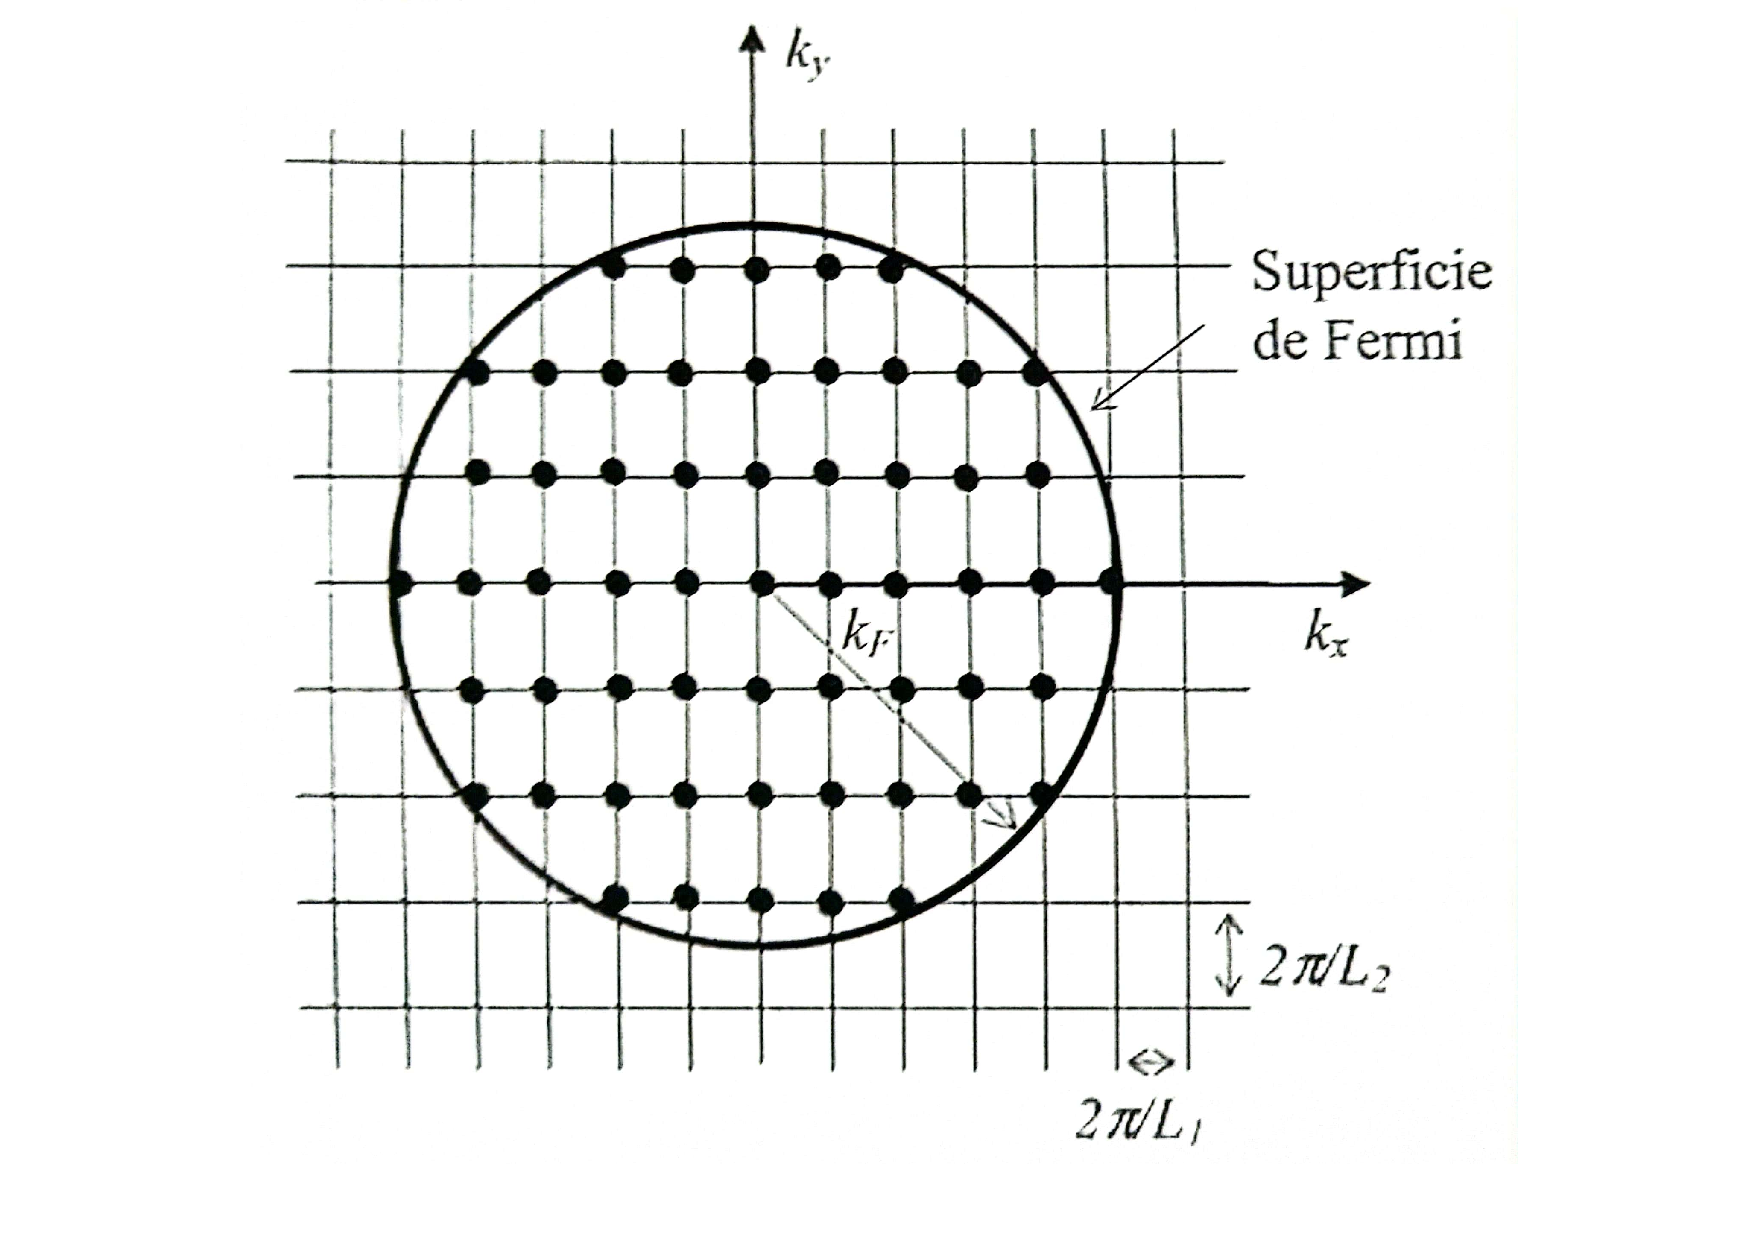
\includegraphics[scale=0.5]{Cuerpo/Ch_04/Fotos libro 1.pdf}
    \caption{Parámetro de red y posiciones de átomos de masa $M$ conectados por una fuerza de constante $C$ enter planos adyacentes. Los desplazamientos de los átomos se designan por $u_{s-1},u_{s},u_{s+1}$.}
    \label{Fig:04-01}
\end{figure}    

\begin{figure}[h!] \centering
    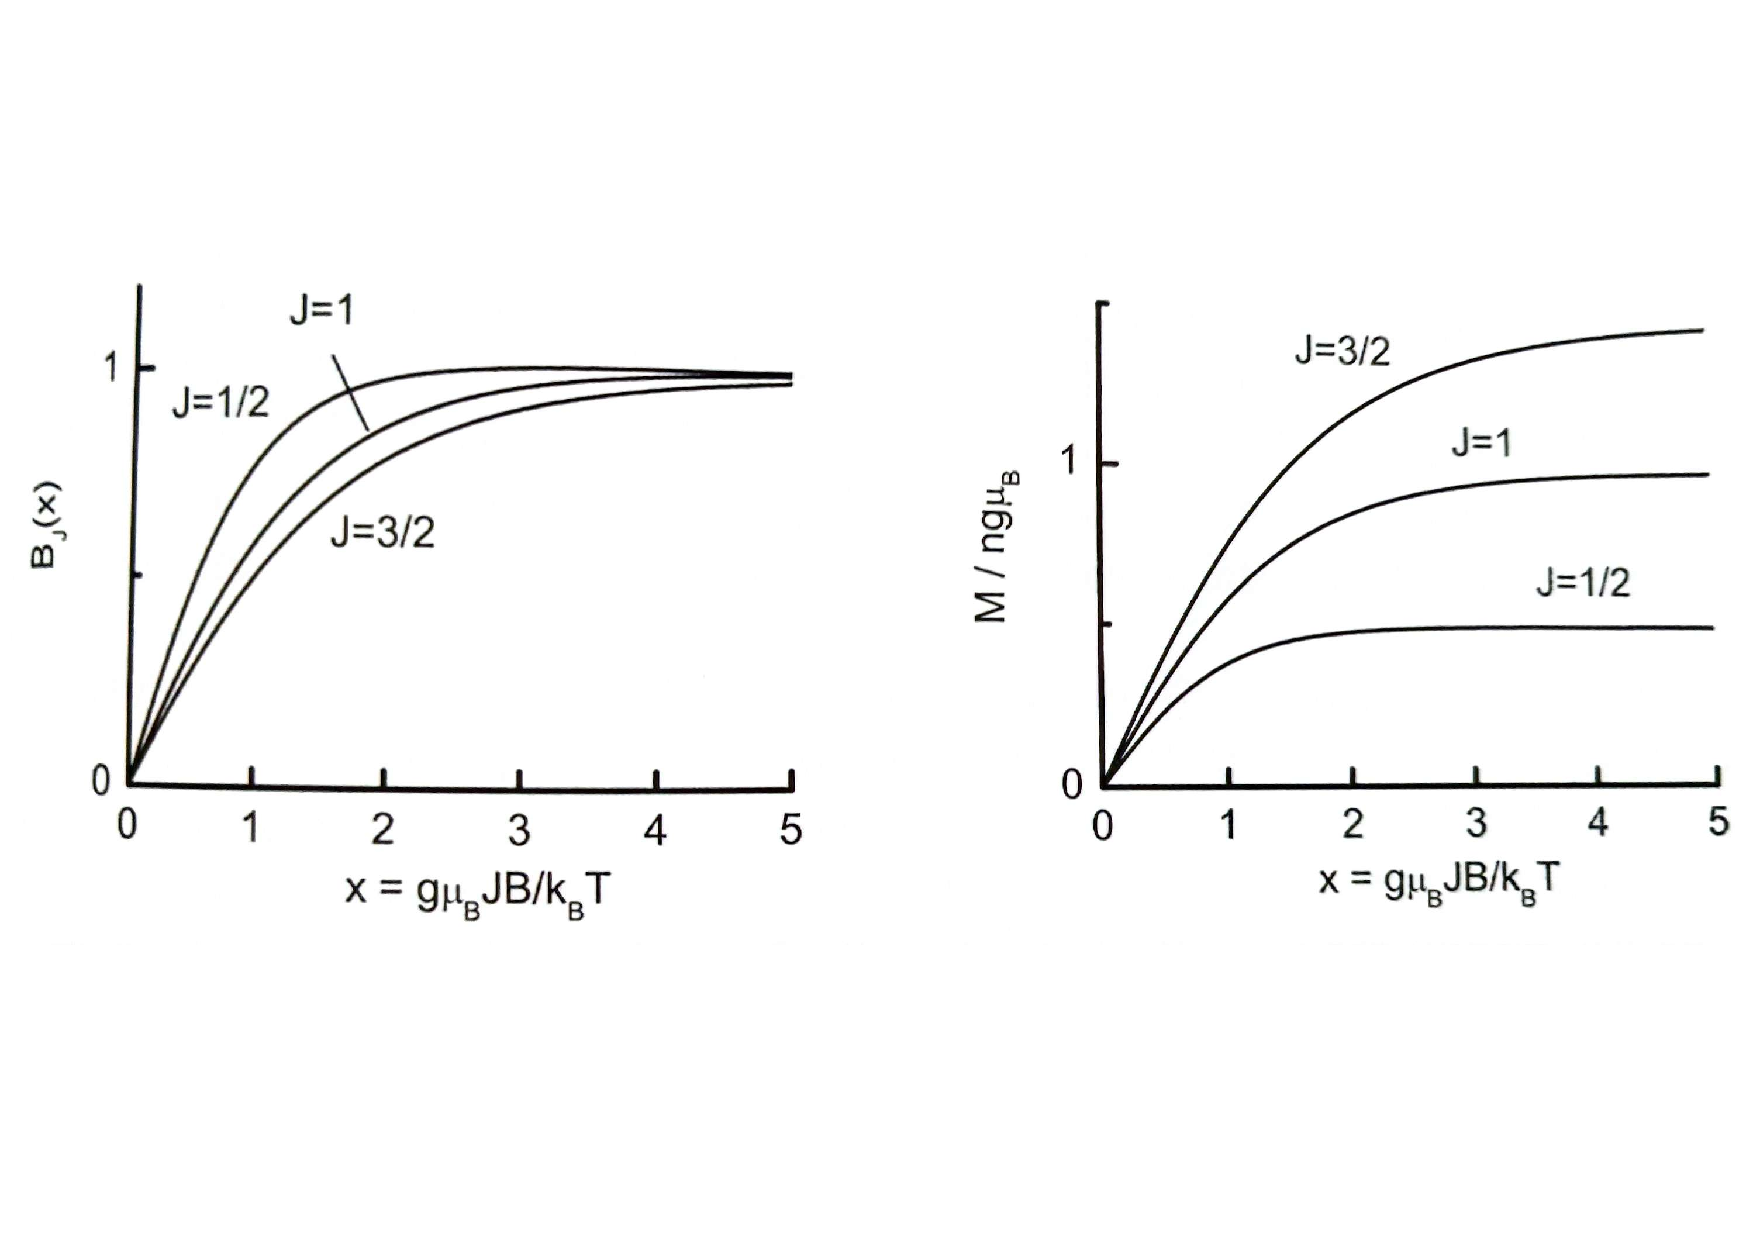
\includegraphics[scale=0.5]{Cuerpo/Ch_04/Fotos libro 2.pdf}
    \caption{Representación de la relación de dipsersión de una cadena monoatómica de átomos de masa $M$ y constante de acoplamiento $C$. Observar que para $k\rightarrow 0$, $\omega \rightarrow k$}
    \label{Fig:04-02}
\end{figure}    

\begin{figure}[h!] \centering
    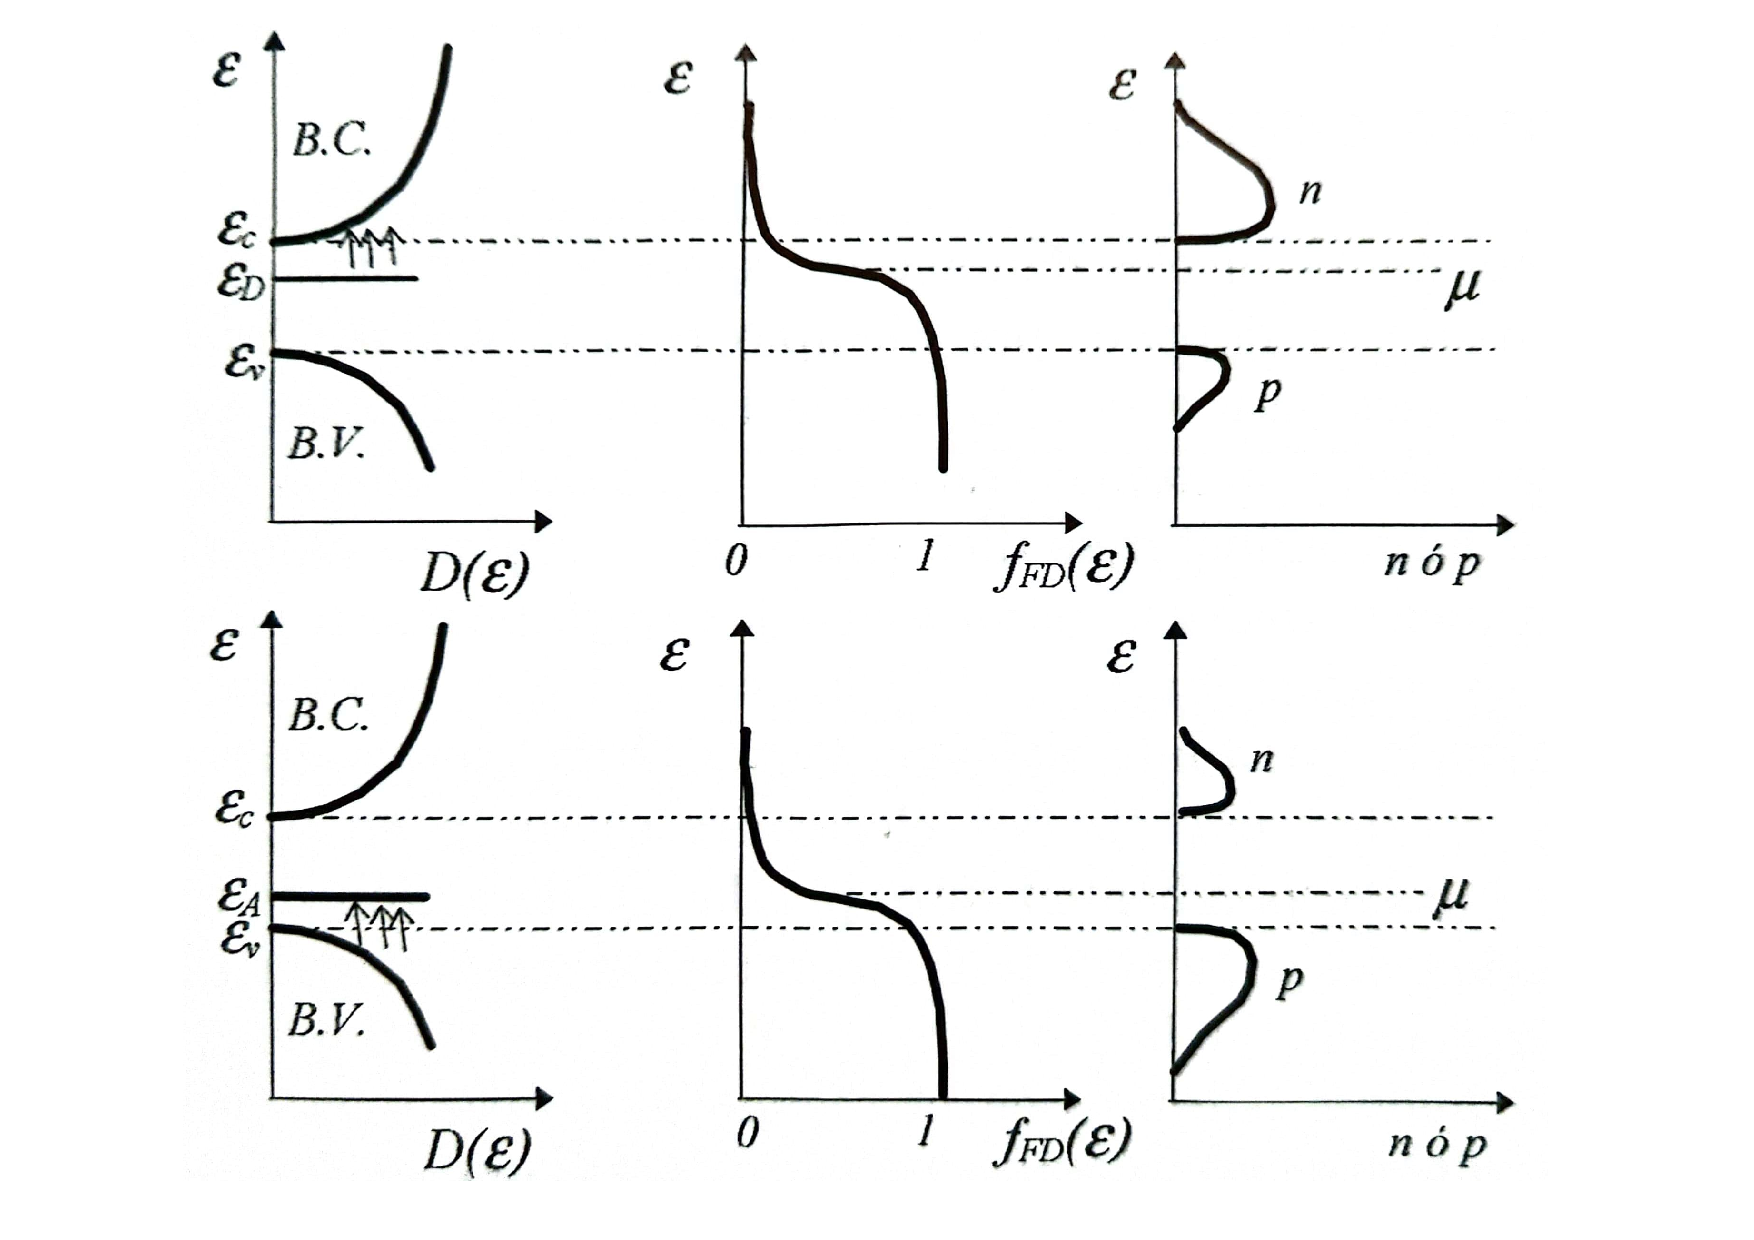
\includegraphics[scale=0.5]{Cuerpo/Ch_04/Fotos libro 3.pdf}
    \caption{Ejemplo de ondas con distancia longitud de onda que sin embargo representan el mismo estado de movimiento de los átomos.}
    \label{Fig:04-03}
\end{figure}    

\subsection{Cristales monoatómicoos tridimensionales}

\section{Vibraciones de cristales con base diatómica}


\subsection{La cadena lineal diatómica}
\begin{figure}[h!] \centering
    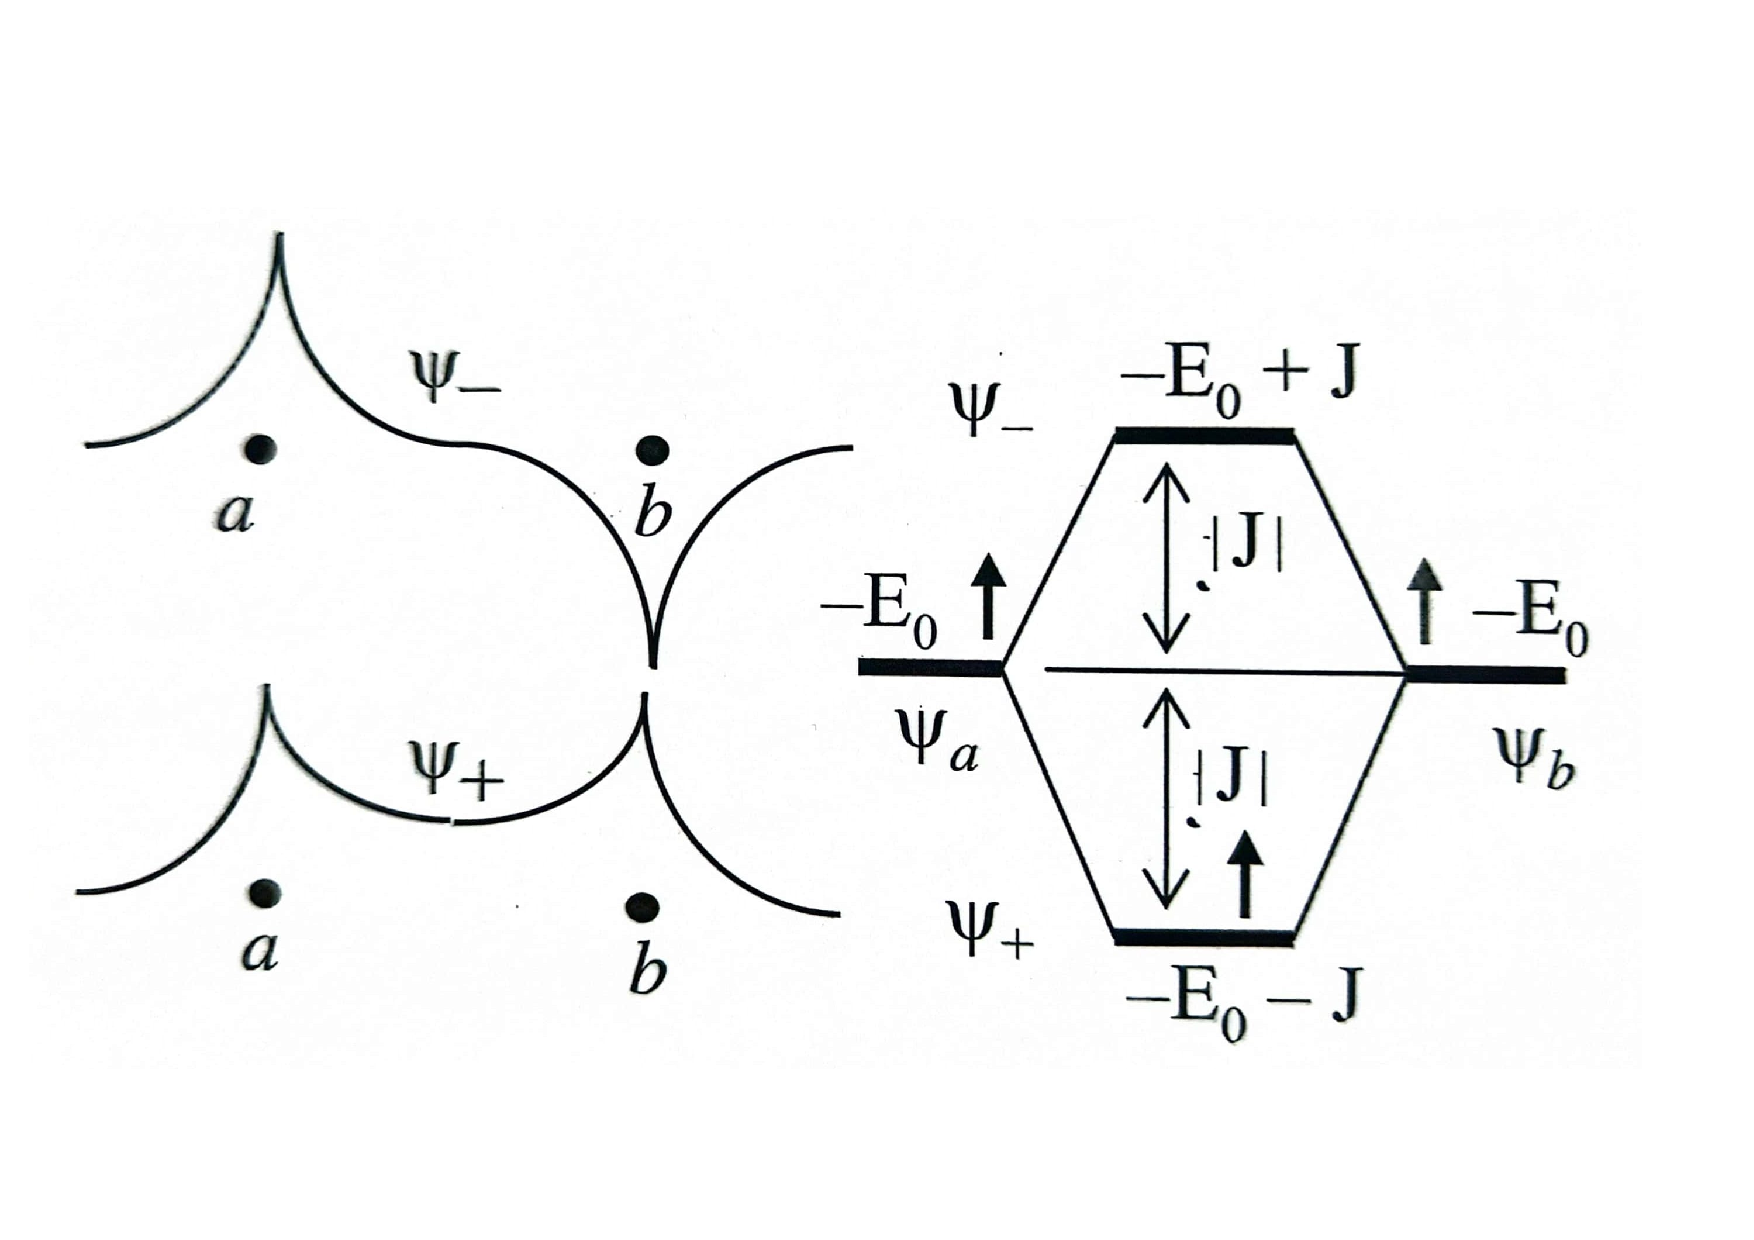
\includegraphics[scale=0.5]{Cuerpo/Ch_04/Fotos libro 4.pdf}
    \caption{Parámetro de red y posiciones de átomos 1 (masa $M_1$) y 2 (masa $M_2$) conectados por una fuerza de constante $C$ entre planos adyacentes. Los desplazamientos de los átomos 1 se designan por $u$ y los átomos 2 por $v$.}
    \label{Fig:04-04}
\end{figure}    

\begin{figure}[h!] \centering
    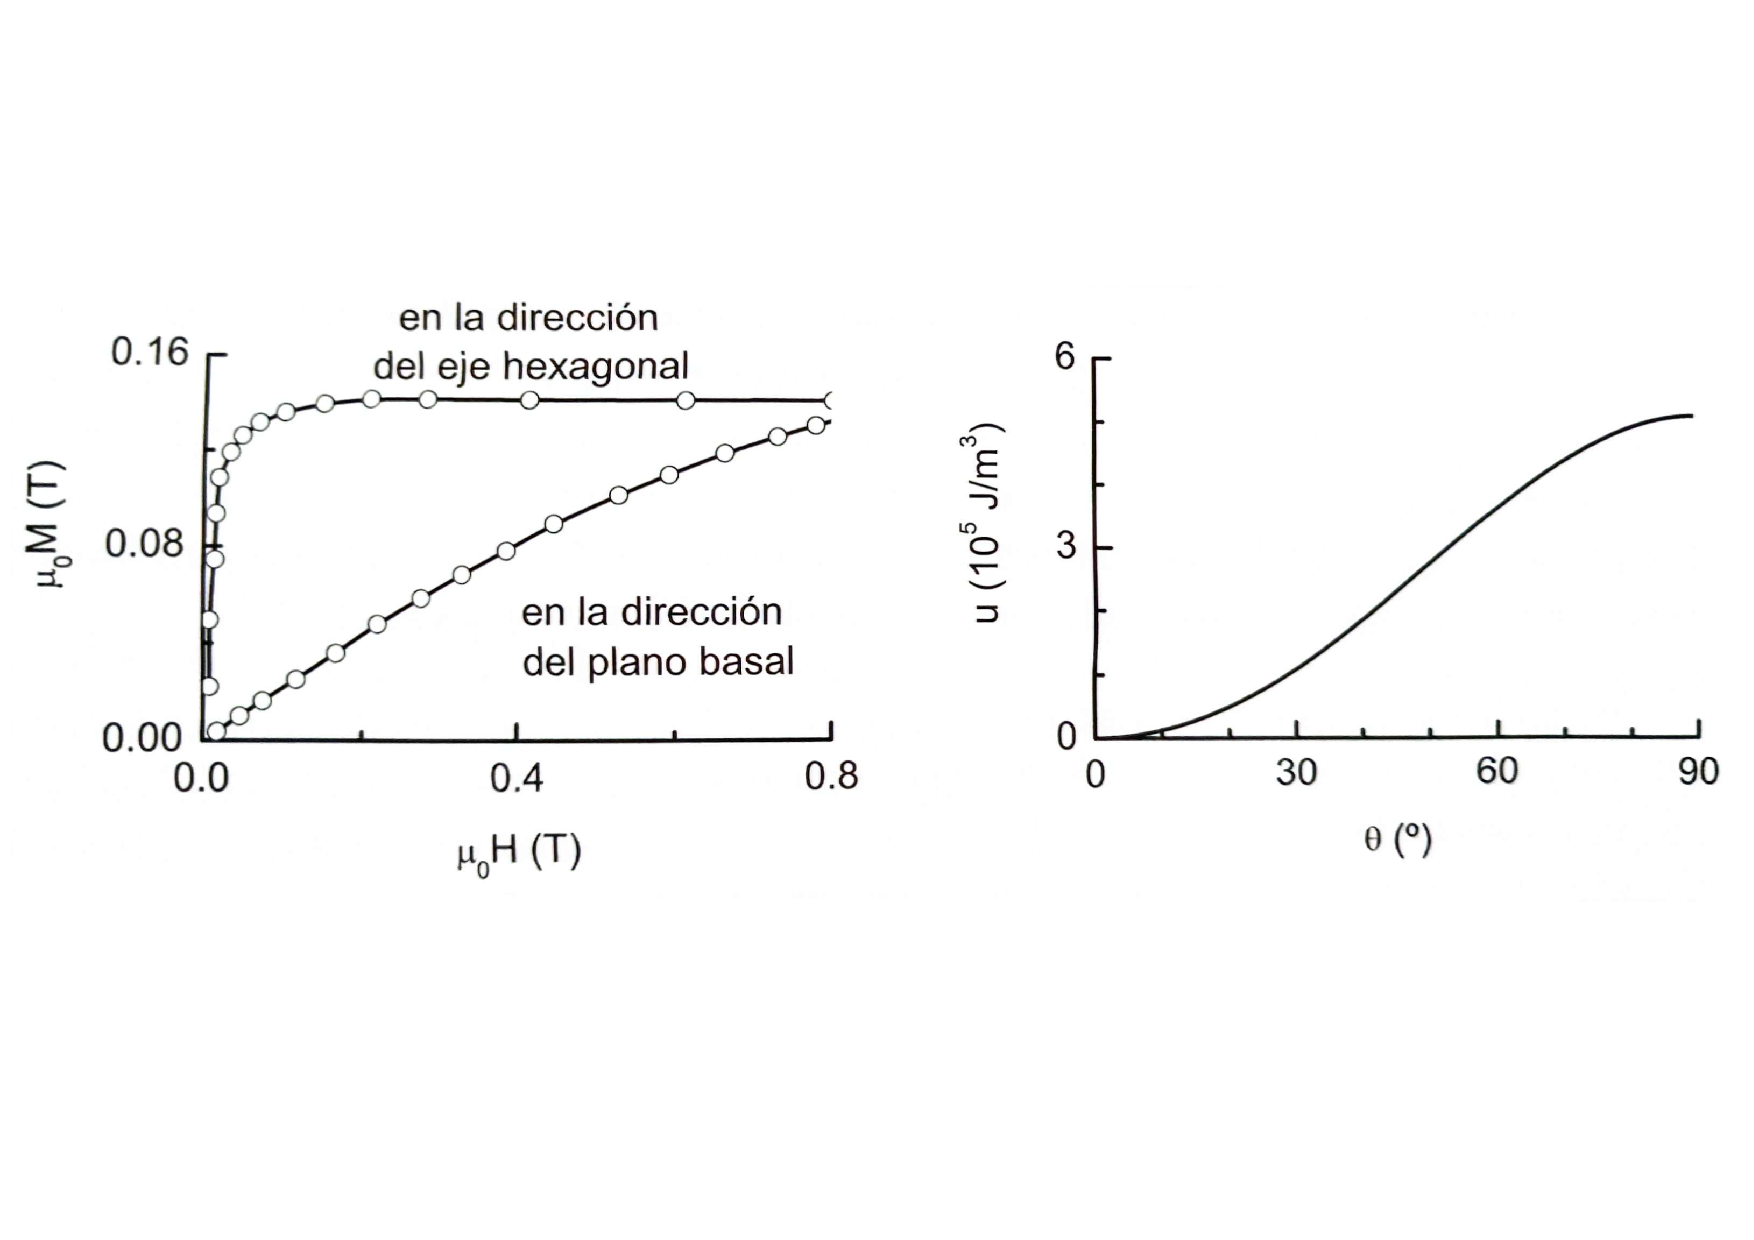
\includegraphics[scale=0.5]{Cuerpo/Ch_04/Fotos libro 5.pdf}
    \caption{Representación de la relación de dipsersión de una cadena diatómica de átomos de masas $M_1$ y $M_2$ y constante de acoplamiento $C$. Observar que para la rama óptica $\omega \rightarrow \text{cte} \neq 0$ cuando $k\rightarrow 0$.}
    \label{Fig:04-05}
\end{figure}    

\begin{figure}[h!] \centering
    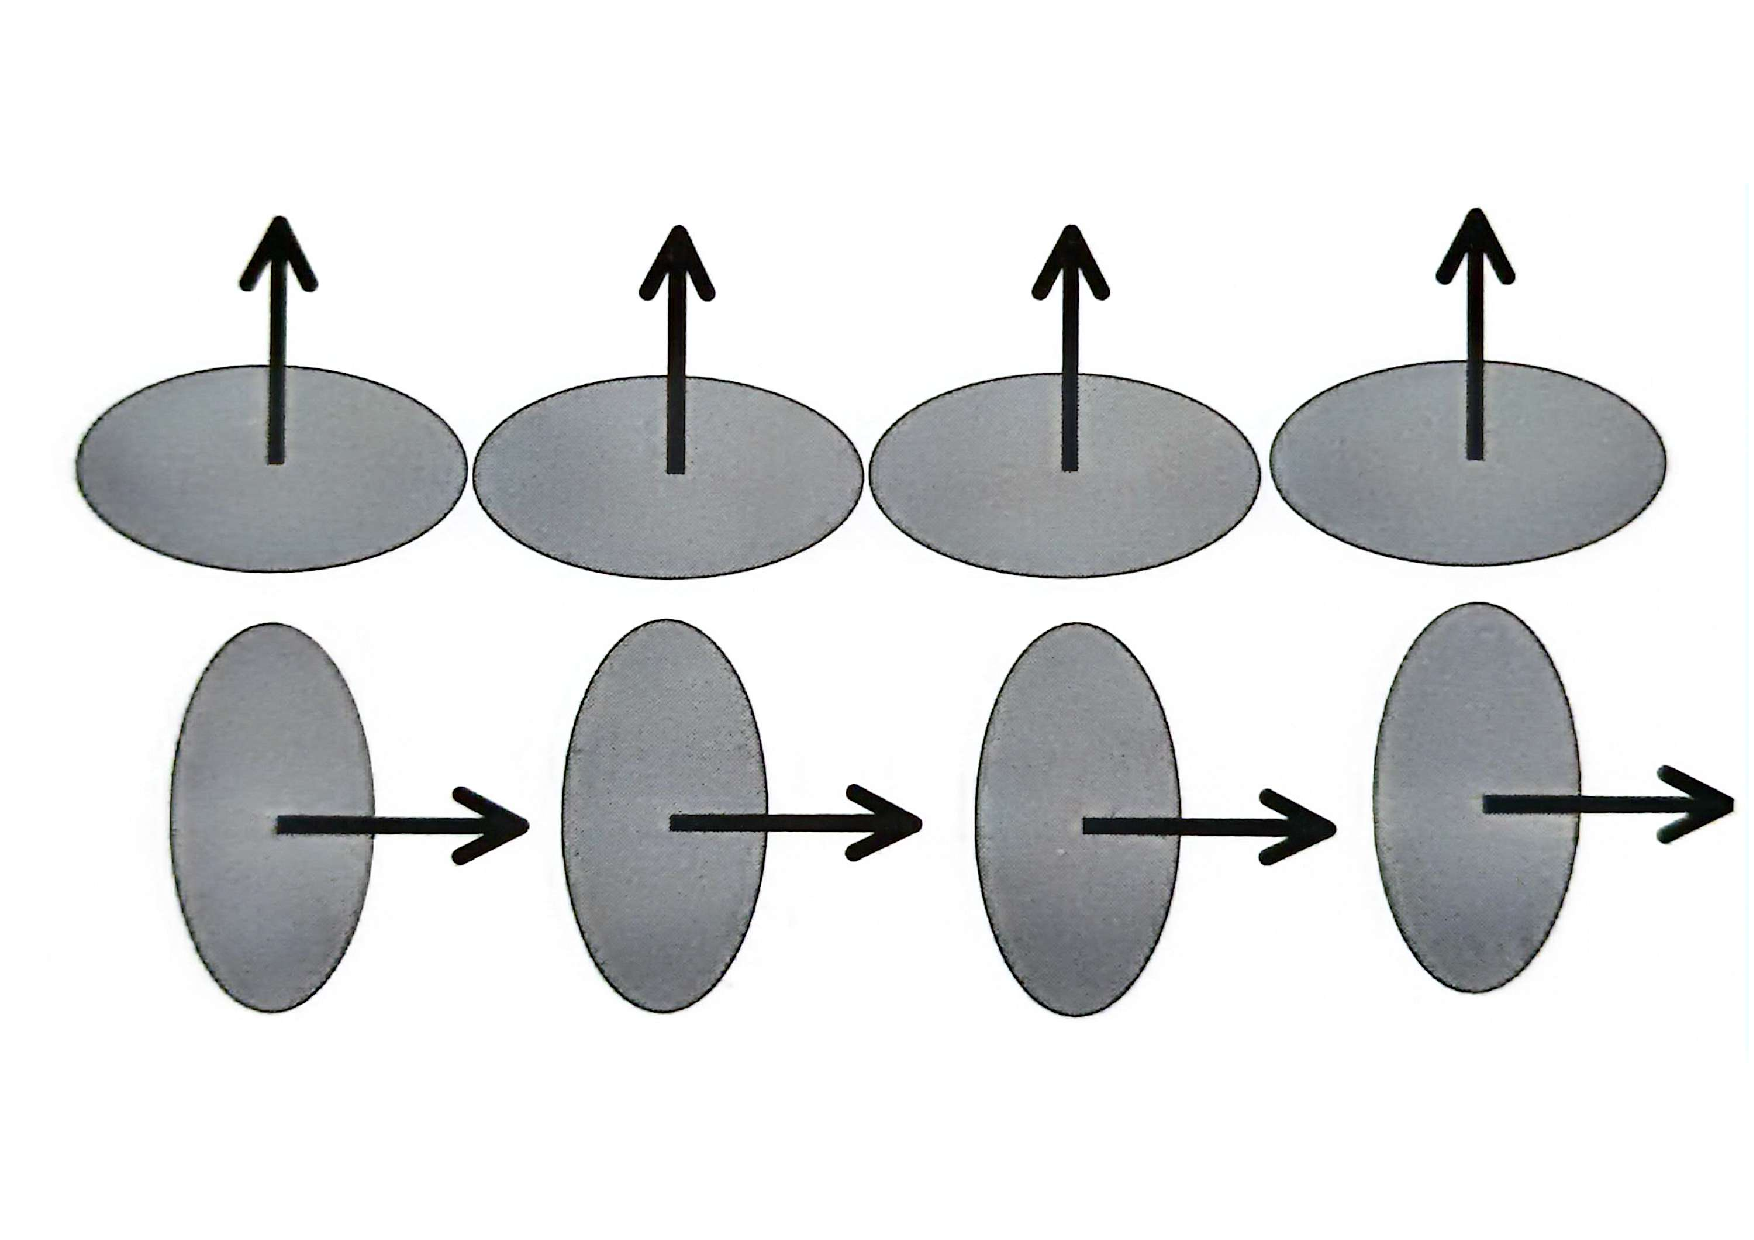
\includegraphics[scale=0.5]{Cuerpo/Ch_04/Fotos libro 6.pdf}
    \caption{Modos óptico y acústica en una cadena diatómica. El desplazamiento atómico respecto a la posición de equilibrio se representa verticalmente.}
    \label{Fig:04-06}
\end{figure}    

\subsection{Cristales tridimensionales poliatómicos}

\begin{figure}[h!] \centering
    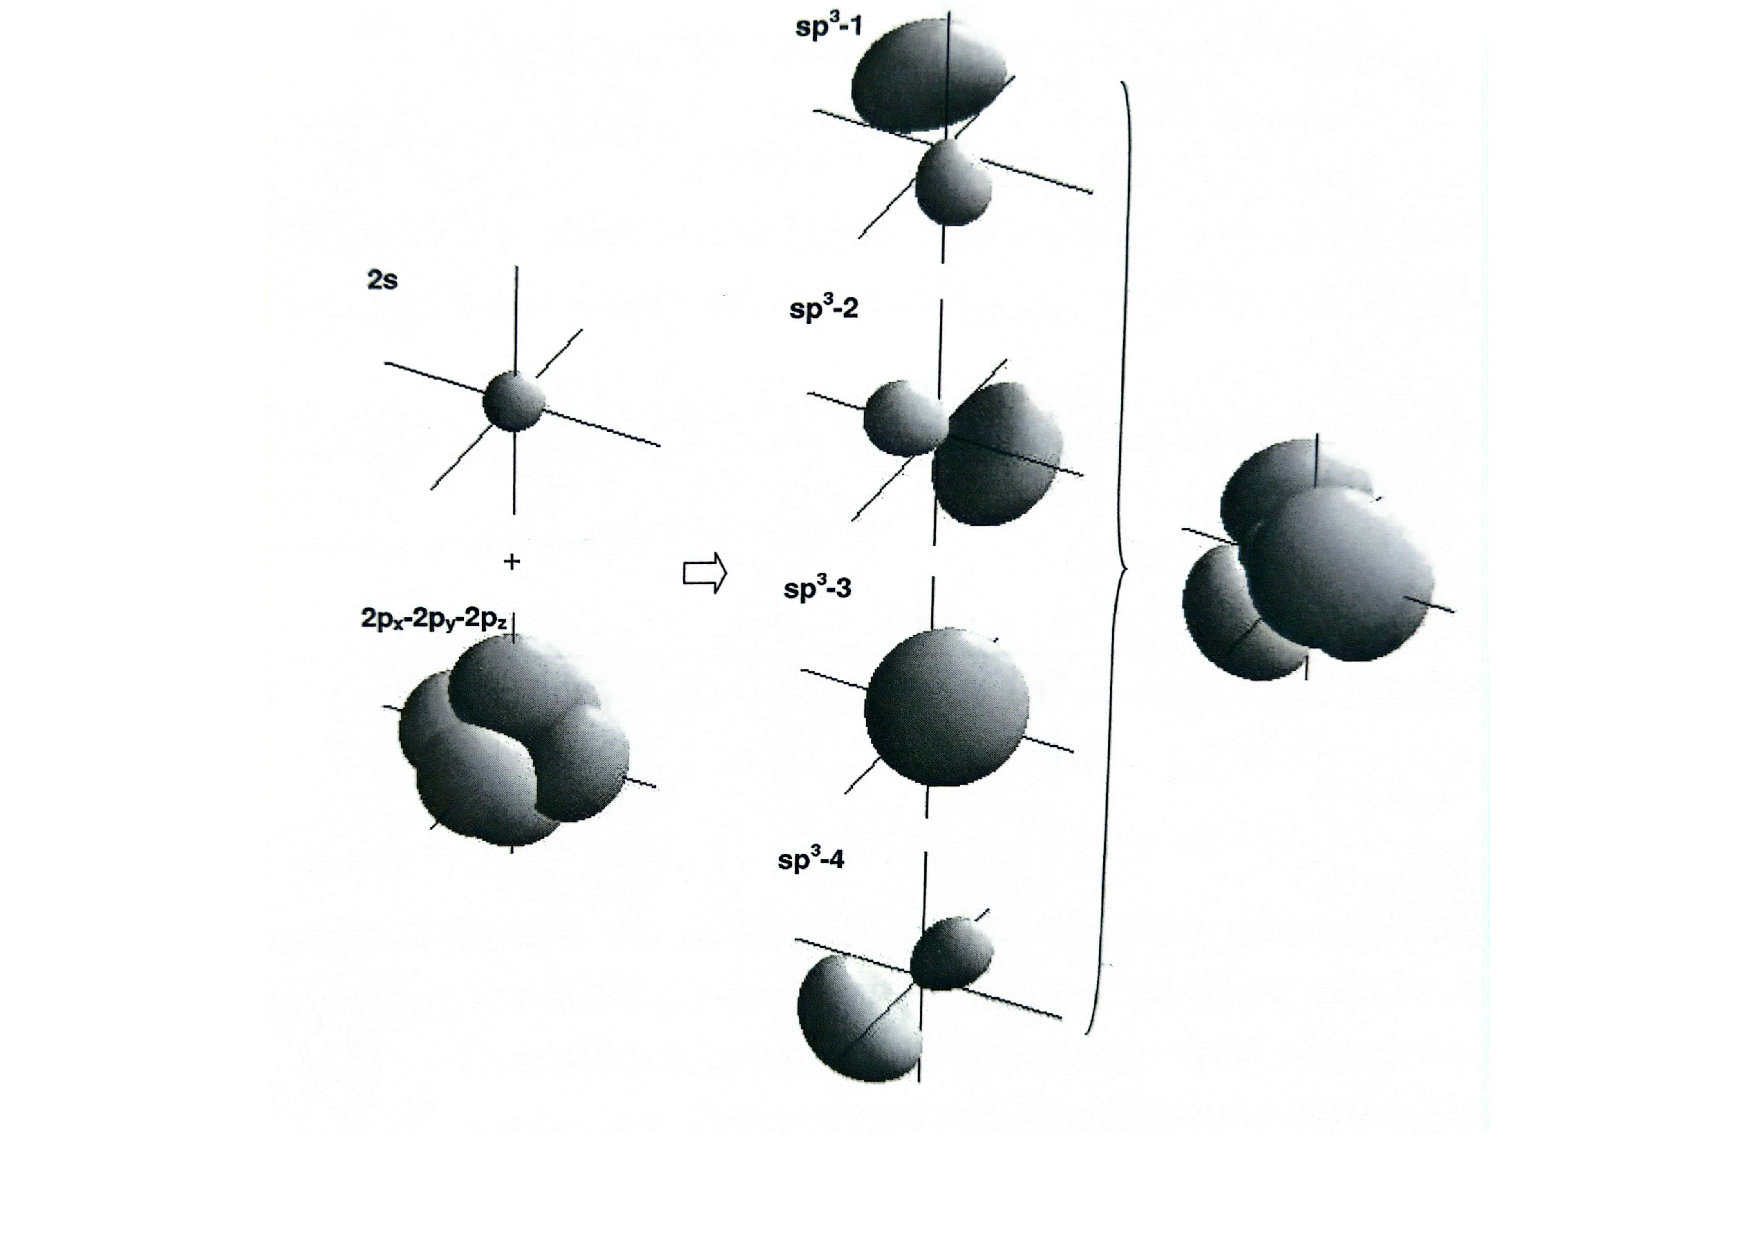
\includegraphics[scale=0.5]{Cuerpo/Ch_04/Fotos libro 7.pdf}
    \caption{Ejemplos de relación de dispersión experiental $\omega (\kn)$. En el eje horizontal se representa $\kn/\kn_{\max}$ para distintas direcciones, y en los ejes verticales la frecuencia $\omega/2\pi$ en undiades de $10^{12}$ Hz.}
    \label{Fig:04-07}
\end{figure}    



\section{Fonones}

\subsection{Cuantización de las ondas elásticas}

\subsection{Espectroscopía de fonones}


\section{Vibraciones de los cristales iónicos}
\begin{figure}[h!] \centering
    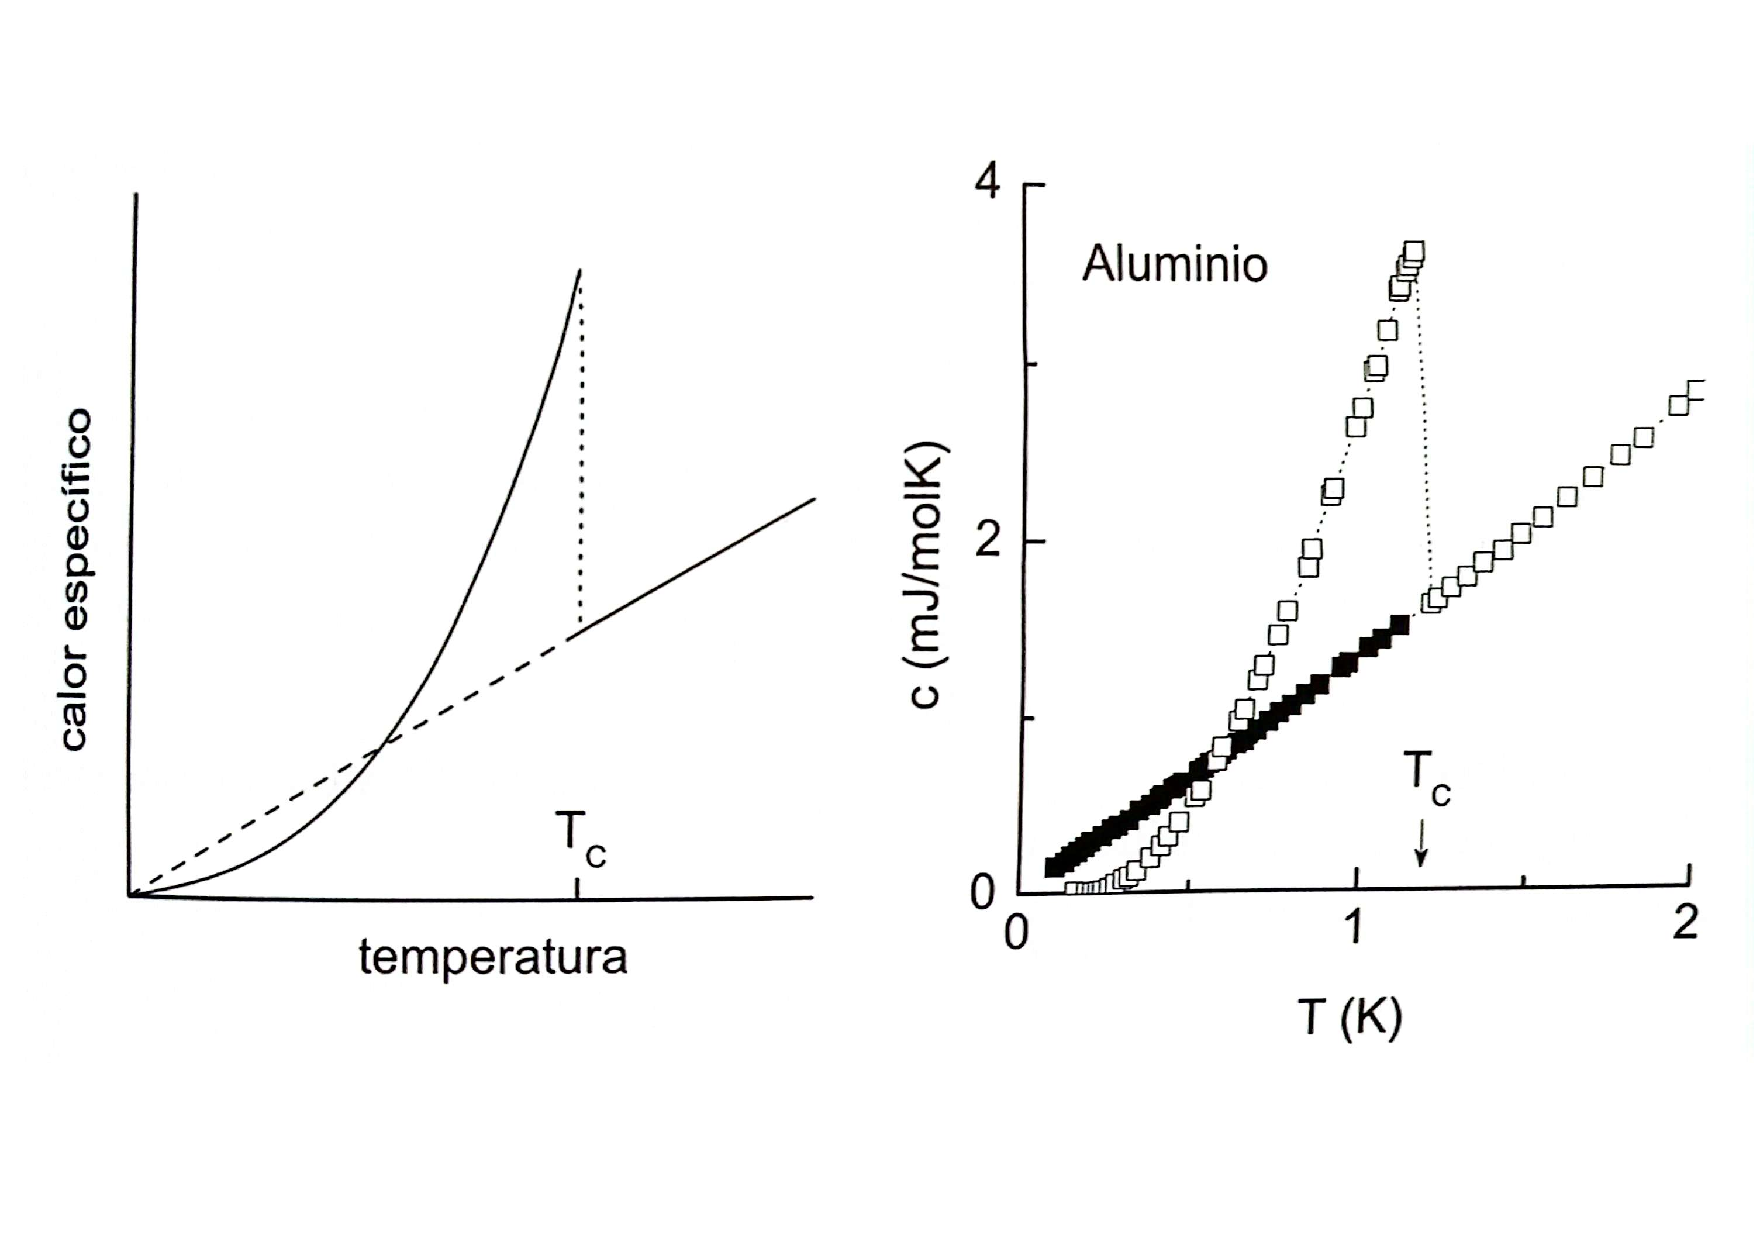
\includegraphics[scale=0.5]{Cuerpo/Ch_04/Fotos libro 8.pdf}
    \caption{(a) Dependencia con la frecuencia de la permitividad eléctrica relativa en cristales iónicos. (b) reflectividad de algunos cristales iónicos para longitudes de odna en el rango infrarrojo.}
    \label{Fig:04-08}
\end{figure}    
